\chapter{Applications des méthodes de descente au deep learning}
\section{Introduction et Motivation}
L'intelligence artificielle représente un ensemble de théories et techniques dont le but est de simuler l'intelligence chez la machine. C'est un concept datant des années 1950 mais qui revient à la mode depuis le début du XXIe siècle, à la fois grâce à des avancées technologiques nombreuses mais également dans les mentalités par le biais de films de science fiction. On peut notamment citer la trilogie Matrix, décrivant un monde dystopique où les machines dominent les hommes après avoir dépassé un stade d'intelligence inattendu. Cependant malgré le fait que l'intelligence artificielle a beaucoup évolué ces dernières années, nous sommes encore loin de ce résultat. Actuellement, les appareils que nous utilisons sont généralement limités à un domaine, par exemple la traduction, la navigation... car les systèmes dit intelligents doivent passer par une phase d'apprentissage. Mais cela pourrait bien changer avec le développement du deep learning ou apprentissage profond.

\subsection{Intelligence artificielle, machine learning et deep learning}
	Mais qu'est-ce que l'apprentissage profond ? C'est en fait un sous-domaine du machine learning, lui même étant une branche de l'intelligence artificielle. Voici une représentation sous forme d'arbres permettant de visualiser différentes approches de l'IA : 
	\begin{figure}[H]
		\centering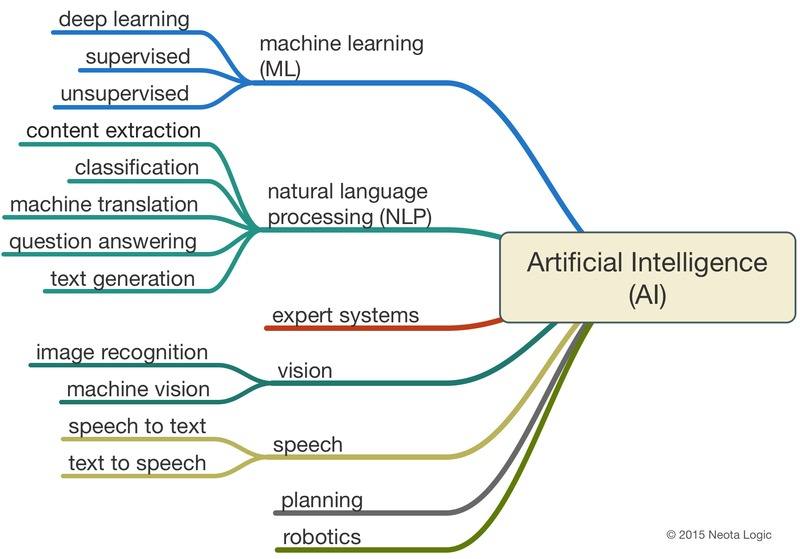
\includegraphics[width=0.7\linewidth]{images/branches}
		\caption{Approches de l'IA}
	\end{figure}
	Pour mieux comprendre ce que sont machine learning et deep learning commençons par les \textit{systèmes experts}. Ce sont des logiciels très spécialisés dont le but est de reproduire la "pensée" d'un expert dans un domaine. Cela permet de remplacer une personne pour une tâche bien précise. Par exemple, le premier système expert mis au point, Dendral (en 1965) permettait d'identifier les consitituants chimiques d'un matériau. Les systèmes experts reposent sur des algorithmes "simples", constitués de conditions "if... then...", pouvant être assimilés à des arbres de décisions. Ils sont donc utilisables uniquement pour des tâches précises et déterminées à l'avance et ne peuvent sortir de leurs bornes d'application. L'apprentissage de la machine est manuelle, c'est l'homme qui doit implémenter toutes les possibilités lui-même.\\
	
	Le machine learning apporte une solution à cela. Dorénavant, l'ordinateur apprend par lui-même. L'homme lui apprend à reconnaitre et à reproduire. On dit qu'on "entraine" la machine. Il faut pour cela lui fournir de grands jeux de données, c'est là qu'intevient le domaine du big data et c'est une des raisons pour lesquelles le développement du machine learning s'est accéléré ces dernières années. Grâce aux données d'entraînement, le programme constitue des données statistiques sur lesquelles il s'appuie ensuite pour faire ses prévisions. \\
	
	Enfin, le deep learning est constitué d'algorithmes permettant au logiciel de s'entrainer lui même. Cette dernière approche est basée sur ce que l'on appelle des "réseaux de neurones" à multiples couches, imitant (plus ou moins) le fonctionnement du cerveau humain. Plus ils reçoivent de données, plus ces réseaux de neurones sont performants. 
	
\section{Architecture d'un réseau de neurones}

\begin{figure}[H]
	\centering
	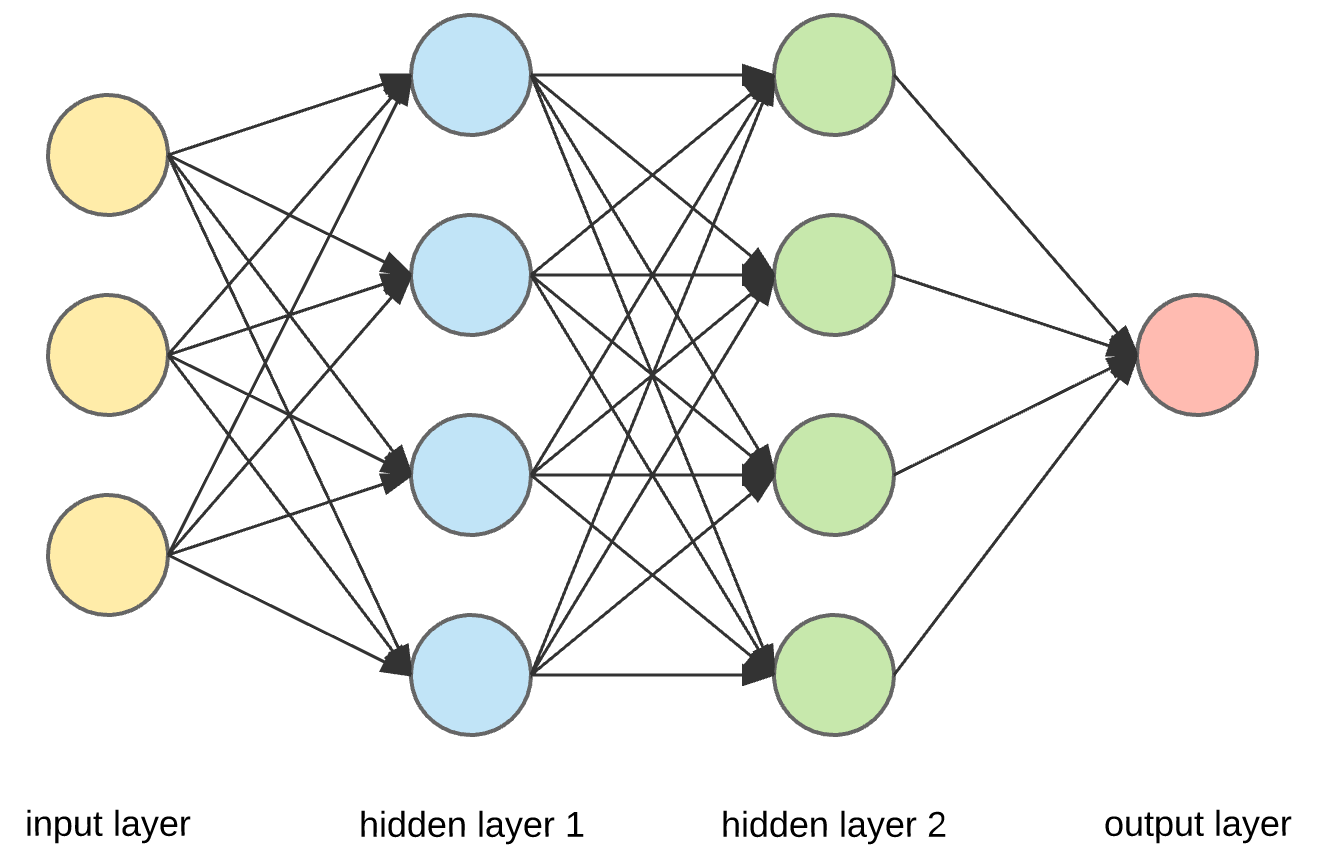
\includegraphics[width=0.75\linewidth]{images/reseau}
	\caption{Architecture}
\end{figure}
	
	
\section{Application des algorithmes}